\documentclass[12pt, a4paper]{article}
\renewcommand*\contentsname{Inhaltsverzeichnis}
\usepackage[ngerman]{babel}
\usepackage{mathptmx}
\usepackage{blindtext}
\usepackage{emptypage}
\usepackage{wrapfig}
\usepackage[pdftex]{graphicx}
\usepackage{geometry}
\usepackage{setspace}
\usepackage{hyperref}
\usepackage[version=4,arrows=pgf-filled,
textfontname=sffamily,
mathfontname=mathsf]{mhchem}
\usepackage[table]{xcolor}
\usepackage{multirow}
\usepackage[table]{xcolor}
\usepackage{array}
\usepackage{float}
\usepackage{mathcomp}
\usepackage{csquotes}
\usepackage[backend=biber,style=chem-acs,sorting=none]{biblatex}
\addbibresource{literatur.bib}  % Deine .bib-Datei einbinden
\renewcommand{\thefootnote}{\fnsymbol{footnote}}

\DeclareCiteCommand{\cite}
  {\usebibmacro{prenote}}
  {\textsuperscript{\printfield{labelnumber}}}
  {\multicitedelim}
  {\usebibmacro{postnote}}


 \geometry{
 a4paper,
 total={170mm,257mm},
 left=25mm,
 top=25mm,
 }
\setstretch{1.213}


\newcommand{\datum}{\day.\month.\year}
\DeclareGraphicsExtensions{.pdf,.jpeg,.png,.jpg} 

\begin{document}


\begin{figure}
    \includegraphics[scale=0.14]{Universität_Bayreuth.svg.png}
\end{figure}


%Deckblatt

{\raggedright Universität Bayreuth\\  95447 Bayreuth}


\vspace{5cm}

\begin{center}
{\LARGE\bf{Anorganische Chemie III}} \\  
\vspace{1cm}
{\Large\bf{Magnetphasen}}\\
\vspace{0.5cm}
{\large Justus Friedrich\\}
{Studiengang: B.Sc. Chemie\\}
{4. Fachsemester}
\end{center}





\thispagestyle{empty}
\begin{center}
{\small Matrikelnummer: 1956010 \\
E–Mail:  bt725206@myubt.de}
\end{center}

\vspace{5cm}

\today


\newpage
%Inhaltsverzeichnis
\tableofcontents
\thispagestyle{empty}


%Teil 1
\newpage
\setcounter{page}{1}
\section{Einleitung}



\subsection{Einführung}


{Magnetismus ist eine Eigenschaft, die auf der Anordnung der Elektronenspins beruht. Diese Spins erzeugen ein magnetisches Moment. Wenn sich die magnetischen Momente innerhalb
 eines Atoms gegenseitig aufheben, ist der Stoff diamagnetisch. Besitzt ein Atom hingegen ein resultierendes magnetisches Moment, ist der Stoff paramagnetisch.\\
\noindent
Paramagnetische Stoffe lassen sich weiter in Ferromagnete, Ferrimagnete und Antiferromagnete unterteilen:
\begin{enumerate}
    \item Bei Ferromagneten richten sich alle magnetischen Momente parallel zueinander aus, wodurch ein starkes makroskopisches Magnetfeld entsteht.
    \item Bei Ferrimagneten sind die magnetischen Momente zwar auch geordnet, jedoch in entgegengesetzten Richtungen mit unterschiedlicher Stärke ausgerichtet. Dadurch bleibt ein resultierendes magnetisches Moment bestehen, das jedoch schwächer ist als bei Ferromagneten.
    \item In Antiferromagneten sind die magnetischen Momente benachbarter Atome entgegengesetzt und gleich stark ausgerichtet, wodurch sie sich gegenseitig vollständig aufheben. Das resultierende magnetische Moment ist somit nazu null.
\end{enumerate}
\noindent
Ziel des Versuchs ist es, Magnetit, Maghemit und Hämatit herzustellen und ihre magnetischen Eigenschaften zu untersuchen. \cite{Skript}
}


\newpage
%Teil2
\section{Durchführung}
\subsection{Darstellung von Magnetit}
Es werden 3.001 g (15.09 mmol) \ce{FeCl2}$\cdot$\ce{4 H2O} in 75 mL Wasser gelöst. Anschließend wird 30 mL einer 1 Molarer (2.599 g/ 65mmol in 65 mL Wasser) NaOH
unter kräftigen Rühren hinzugegeben. Nach 35 min wird der Niederschlag abgenutscht und getrocknet.

\subsection{Darstellung von Maghemit}
Ein Teil des Hergestellten Magnetits wird für 2 h bei 250 °C getempert.

\subsection{Darstellung von Hämatit}
Ein Teil des Maghemit wird für 10 h bei 700°C getempert.\footnote{Hier sollte eigentlich nur für 2 h getempert werden, aufgrund eines Fehlers wurde für 10 h getempert.}


\newpage
\section{Auswertung}
\subsection{Phasenanalyse von Magnetit}

Da bei der verwendeten Wellenlänge der Röntgenquelle eine starke Fluoreszenz von Eisen auftritt, konnten keine eigenen XRD-Messungen an den hergestellten Substanzen durchgeführt werden. 
Um dennoch eine Vergleichsbasis zur Interpretation zu schaffen, wurde ein Referenzdiffraktogramm von Magnetit herangezogen.
Die Beispielmessung ist in Abbildung \Ref{Magnetitxrd} dargestellt. 

\noindent
Bei der Analyse der XRD-Daten zeigte sich eine Vertauschung der Dateinamen: Die Datei „Magnetit“ enthält das Diffraktogramm von Maghemit, und „Maghemit“ jenes von Magnetit. Diese Verwechslung wurde im Protokoll berücksichtigt, sodass die Dateien im Folgenden entsprechend korrigiert zugeordnet werden.
\begin{figure}[!h]
    \centering
    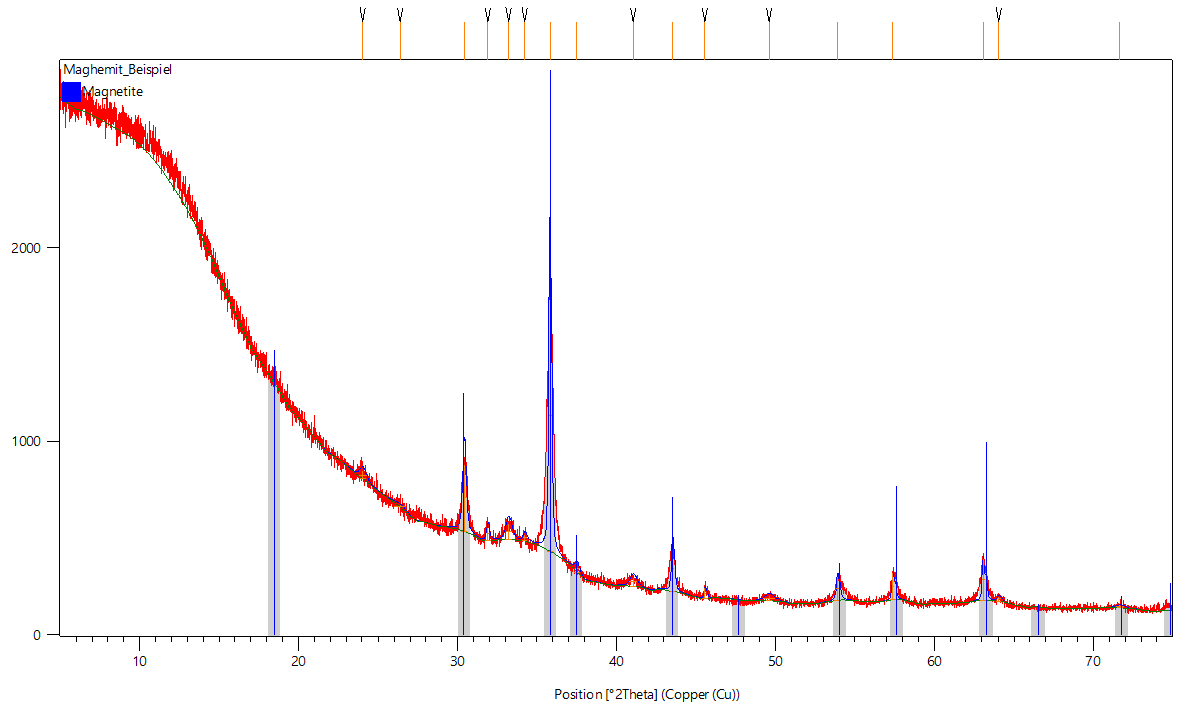
\includegraphics[width=0.8\linewidth]{Magnetit.png}
    \caption{Das XRD-Diagramm zeigt Magnetit mit den Referenzreflexen gemäß dem Referenzcode 01-075-0449.}
    \label{Magnetitxrd}
\end{figure}

\noindent
Als Hauptphase wurde mit 67 \% kubisches Magnetit identifiziert (\textit{HighScore Plus} Score 54, Referenzcode 01-075-0449); als Nebenphase wurde mit 33 \% rhomboedrisches \ce{Fe2O3} bestimmt (\textit{HighScore Plus} Score 17, Referenzcode 01-073-2234).
Anschließend wird die Theoretische Elementarzelle mit der Festgestellten Elementarzelle verglichen. Dies wird in der Tabelle \ref{Kastenlängemagnetit} dargestellt.
\newpage
\begin{table}[h!]
\caption{\textit{Zeigt die Theoretische und Festgestellte verfeinerte Einheitszelle von den hergestellten Magnetit (Referenzcode 01-075-0449). Die Verfeinerung wurde mithilfe des Programmes HighScore Plus durchgeführt. }}
\begin{center}
\begin{tabular}{|>{\columncolor{lightgray}}p{4cm}|>{\centering\arraybackslash}p{4cm}|>{\centering\arraybackslash}p{4cm}|}
   \hline
   \rowcolor{gray}
   &Theoretische Elementarzelle& Festgestellte verfeinerte Elementarzelle (Standardabweichung) \\
   \hline
   a[\AA]& 8.3100& 8.324 (3)\\
   \hline
   b[\AA]&8.3100& 8.324 (3)\\
   \hline
   c[\AA]&8.3100& 8.324 (3)\\
   \hline
   $\alpha$[°]&90& 90\\
   \hline
   $\beta$[°]&90& 90\\
   \hline
   $\gamma$[°]&90& 90\\
   \hline
   Volumen[\AA$^3$]&573.86 & 576.68\\
   \hline
    Chi Square&\multicolumn{2}{c|}{4.270028 $\cdot 10^{-6}$}\\
   \hline
   Synder`s FOM&\multicolumn{2}{c|}{9.4929}\\
\hline
\end{tabular}
\label{Kastenlängemagnetit}
\end{center}
\end{table}

\noindent
Aus Tabelle \ref{Kastenlängemagnetit} lässt sich erkennen, dass die Elementarzellen nicht vollständig übereinstimmen. Dies liegt wahrscheinlich an der \ce{Fe2O3}-Verunreinigung.

\subsection{Phasenanalyse von Maghemit}


\newpage
\section{Zusammenfassung}




\newpage
\section{Literaturverzeichnis}
\printbibliography







\end{document}